\documentclass[conference]{inc/IEEEtran}
\IEEEoverridecommandlockouts
% The preceding line is only needed to identify funding in the first footnote. If that is unneeded, please comment it out.
% !TeX root = ../main.tex
\usepackage{a4wide}

\usepackage[utf8]{inputenc}

%\usepackage[ngerman]{babel}
\usepackage[english]{babel}

\usepackage[T1]{fontenc}
\usepackage{palatino}
\usepackage{cite}
\usepackage{graphicx}
\usepackage{caption}
\usepackage{url}
\usepackage{acronym}
\usepackage{tocloft}
\usepackage{algorithmic}
\usepackage{mathpazo}
\usepackage{amsmath}
\usepackage{amsfonts}
\usepackage{adjustbox}
\usepackage{textcomp}
%\usepackage{subcaption}

\usepackage{hhline}
\usepackage{fancyhdr}
\usepackage{amssymb}
\usepackage{floatflt}
\usepackage{setspace}
\usepackage{float}
\usepackage{booktabs}
\usepackage{color}
\usepackage{listings}
\usepackage{array}
\usepackage{scrhack}
\usepackage{xcolor}
\usepackage{wrapfig}
\usepackage[hidelinks]{hyperref}
\usepackage{url}
\usepackage{lmodern}
\usepackage{multirow}
\usepackage{subfig}
\usepackage{cleveref}
\usepackage{lipsum}
\usepackage[bottom, hang]{footmisc}


\def\BibTeX{{\rm B\kern-.05em{\sc i\kern-.025em b}\kern-.08em
    T\kern-.1667em\lower.7ex\hbox{E}\kern-.125emX}}
\begin{document}

\title{Neural Network-Based Iris Classification and Genetic Algorithm-Driven SHUBERT Function Optimisation \\
{\footnotesize Completed as part of \textit{M25352 Neural Networks and Genetic Algorithms}}
}


\author{\IEEEauthorblockN{Connor Brook}
  \IEEEauthorblockA{\textit{BSc. Data Science and Analytics} \\
    \textit{University of Portsmouth}\\
    Portsmouth, United Kingdom \\
    brook@connordata.science}
  \and
  \IEEEauthorblockN{Jamie Doe}
  \IEEEauthorblockA{\textit{BSc. Software Engineering} \\
    \textit{University of Portsmouth}\\
    Portsmouth, United Kingdom \\
    UP953068@myport.ac.uk}
}

\maketitle

\begin{abstract}
  In this paper, we explore two different optimisation problems: a neural network for the Iris dataset and a genetic algorithm for the SHUBERT function. We design, implement, and evaluate both optimisation techniques, comparing their performance and discussing the advantages and disadvantages of each method. The artificial neural network is employed to classify iris flowers based on their morphological features, while the genetic algorithm is utilized to optimize the SHUBERT function, a well-known benchmark problem in the global optimisation domain. By comparing the results of these two distinct optimisation approaches, we provide insights into their applicability and effectiveness in solving different types of problems.
\end{abstract}

\section{Introduction}

Optimisation techniques like artificial neural networks (ANNs) and genetic algorithms (GAs) have become prevalent due to their broad applications, including machine learning and finance. This paper applies ANNs for Iris dataset classification and GAs for SHUBERT function optimisation, both complex problems in their respective fields. The comparison of these methods aims to elucidate their strengths, weaknesses, and suitability for different problem types, encompassing their design, implementation, and evaluation.

\section{Part I: Neural Networks for Classification/Mapping Task}

\subsection{Introduction}

The Iris dataset, a standard problem in machine learning introduced by Ronald A. Fisher in 1936, is the focus of this coursework. Our aim is to build an artificial neural network capable of classifying Iris plants into one of three species: Iris Setosa, Iris Versicolour, and Iris Virginica. We address the issue of non-linear separability between the species by employing a comprehensive approach that includes data preprocessing, designing the neural network, optimization, and finally, validation and evaluation. This project offers a practical experience in implementing a neural network and provides an understanding of its role in solving classification problems.

\subsection{Data Analysis and Pre-processing}

\subsubsection{Data Analysis}

The first step in our approach involves a detailed analysis of the Iris dataset. We employ a variety of visualization techniques to uncover the relationships among attributes and the distribution of different Iris species. This is crucial in the design of the ANN's architecture.

\begin{figure}
  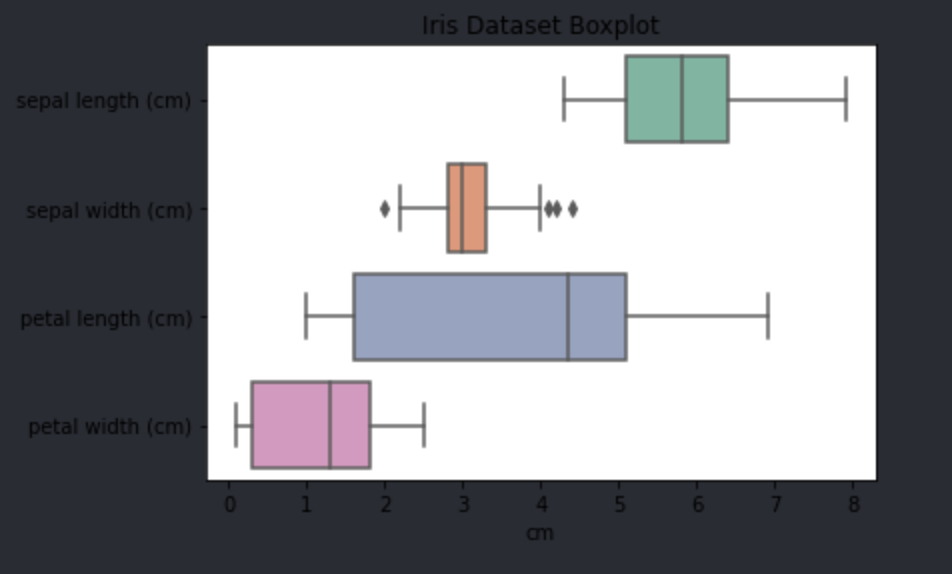
\includegraphics[width=0.4\textwidth]{figures/boxplot.png}
  \caption{Boxplot}
  \label{fig:boat1}
\end{figure}

\textbf{Boxplot}: We construct a boxplot to visualise the distribution of each attribute (sepal length, sepal width, petal length, and petal width), done to display the central tendency and dispersion of the data. No outliers are observed within the dataset.

\textbf{Pairplot}: We also generate a pairplot, which offers a holistic view of relationships between all possible pairs of attributes. This scatterplot matrix allows us to observe the linear separability of the Iris Setosa species from the other two. However, it also highlights the substantial overlap between Iris Versicolour and Iris Virginica, which indicates a potential challenge in the classification task

\begin{figure}
  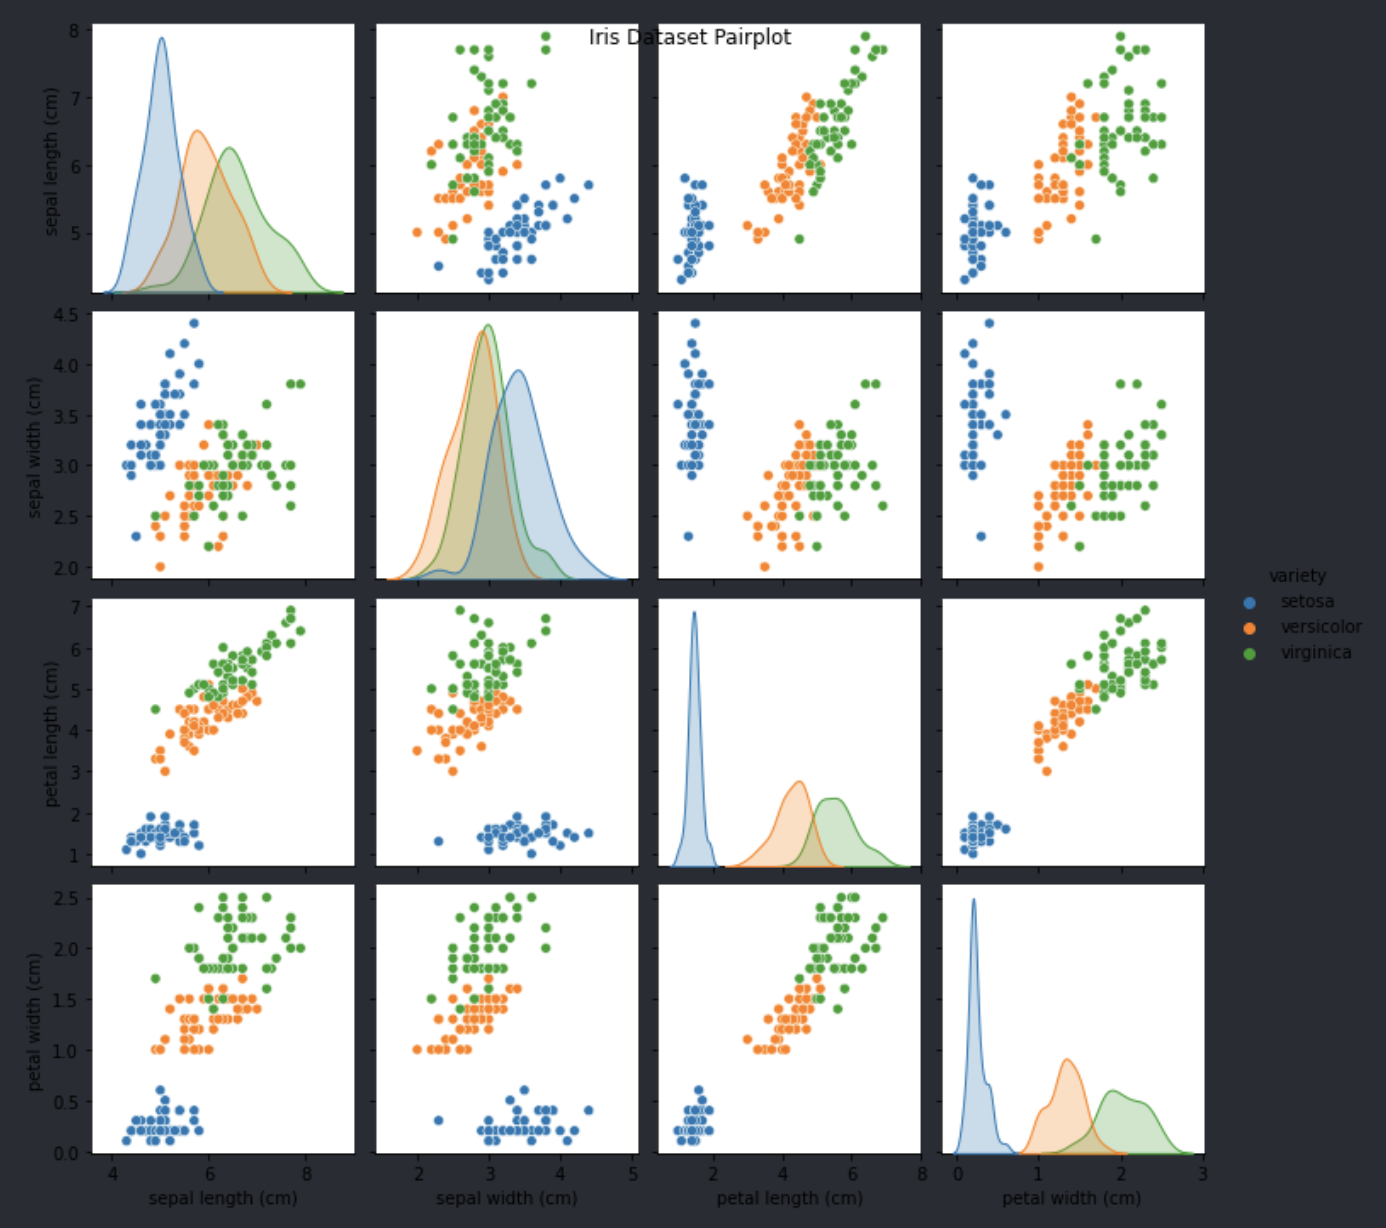
\includegraphics[width=0.4\textwidth]{figures/pairplot.png}
  \caption{Pairplot}
  \label{fig:boat1}
\end{figure}

\textbf{Correlation Matrix}: To quantify the linear relationships between the attributes, we compute a correlation matrix. We represent this matrix as a heatmap, which facilitates the identification of strong correlations. Notably, we observe strong positive correlations between petal length and petal width, and between petal length and sepal length. These correlations are expected, as the petal length and width are highly dependent on the sepal length.

\begin{figure}
  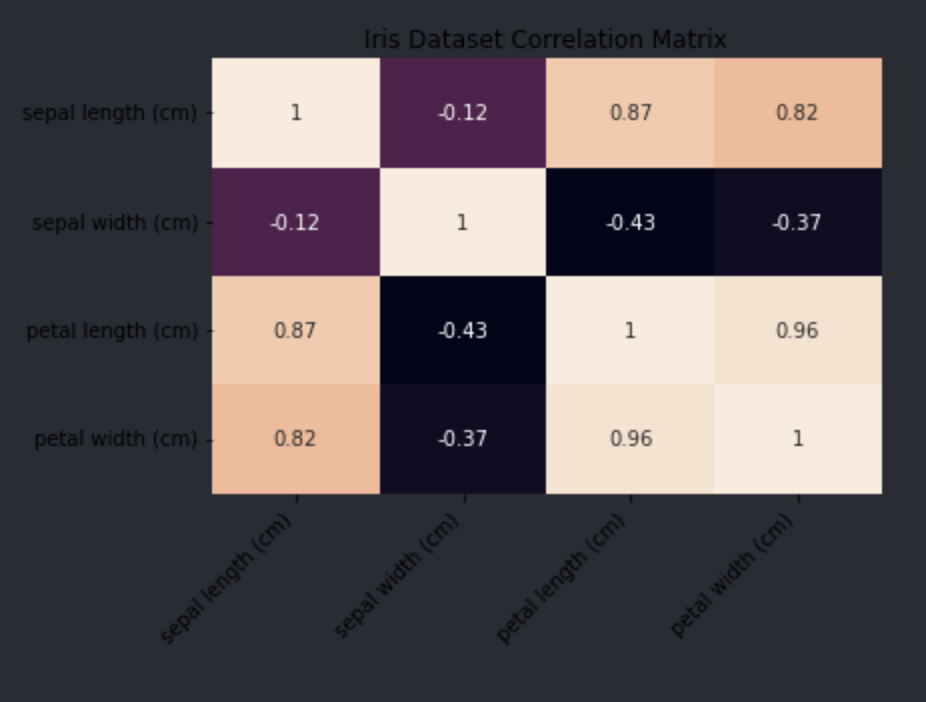
\includegraphics[width=0.4\textwidth]{figures/correlationmatrix.png}
  \caption{Correlation Matrix}
  \label{fig:boat1}
\end{figure}


\textbf{Principal Component Analysis (PCA)}: To better visualise the dataset and potentially simplify the learning task, we perform PCA with three components. This technique reduces the dimensionality of the dataset and projects the data onto a lower-dimensional space. We then use a 3D scatterplot to visualize the clustering of the Iris species in this reduced space, providing further visualisation of the linear separability of Setosa and the overlap between Versicolour and Virginica.

\begin{figure}
  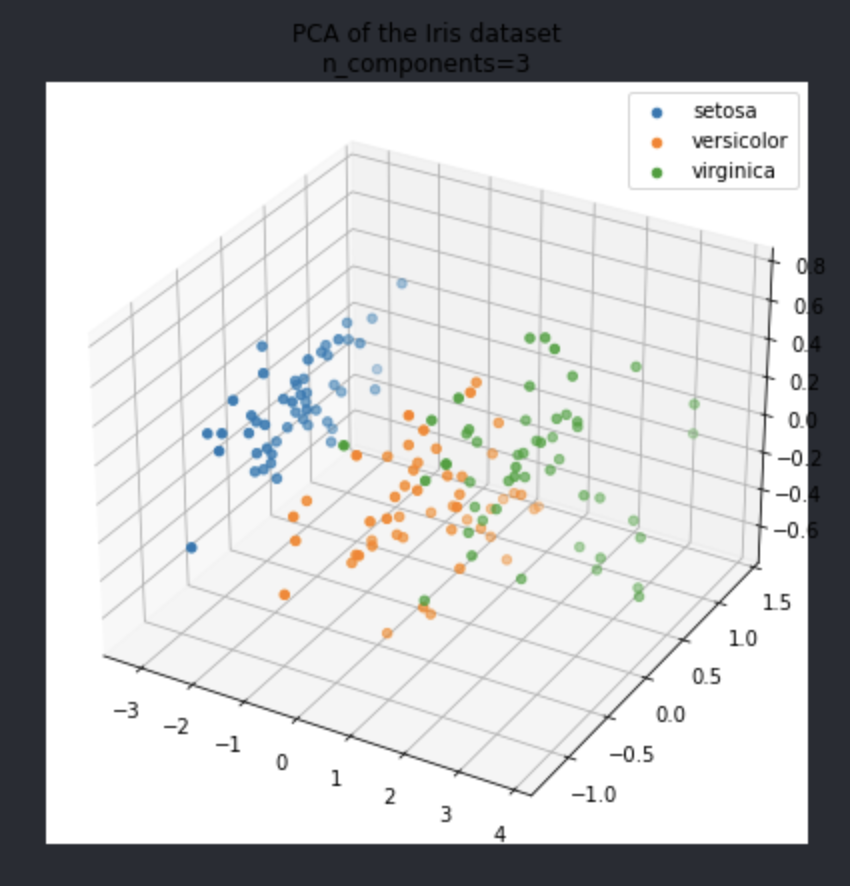
\includegraphics[width=0.4\textwidth]{figures/pca.png}
  \caption{PCA Scatterplot}
  \label{fig:boat1}
\end{figure}

\subsubsection{Data Pre-processing}

Having gained a thorough understanding of the dataset's structure, we proceed to pre-process the data to ensure it is appropriately prepared for neural network training.

\textbf{Splitting the dataset}: We split the Iris dataset into training, validation, and testing sets, using a 50\%:20\%:30\% ratio respectively. This division is critical as it ensures different sets of data for different purposes. The training set is used to train the model, the validation set fine-tunes the model parameters, and the testing set provides a final evaluation of the model's performance on unseen data. This segregation prevents overfitting and helps us create a model that can generalize well to new data.

\textbf{Data standardization}: To prevent features with larger values from dominating the objective function, we scale the data to have zero mean and unit variance. This standardization technique is a common practice in machine learning as it ensures all features contribute equally to the model's learning.

\textbf{One-hot encoding}: To handle categorical features, we perform one-hot encoding. This process transforms categorical features into binary vectors, ensuring that the model does not interpret these categorical features as ordinal which could lead to the network incorrectly inferring hierarchical relationships between categories.

\subsection{Network Design and Structure}


\subsubsection{Network Overview}

Our ANN has been custom-built to address the classification task using the Iris dataset. The network's input layer features four nodes, each corresponding to the unique attributes found in the Iris dataset, namely sepal length, sepal width, petal length, and petal width.

The architecture of the ANN is deep and layered, with a hidden dimension of 64 and 12 layers in total, allowing for more complex representations. The output layer, the final segment of the network, consists of three nodes that correspond to the three Iris species. The prediction is considered by applying softmax to the output layer, which converts the output values into probabilities that sum to one. The node with the highest probability is then selected as the predicted class.

The activation function chosen for our network is GELU, as it allows gradients to propagate, enabling more nuance in the learning process. GELU, performs better than  RELU and ELU on MNIST, especially when combined with dropout, making it an excellent choice for handling noisy data. This choice is backed by the study by
% Hendrycks, D., & Gimpel, K. \(2016\) as referenced in the text.

To further enhance learning and prevent overfitting, we have integrated dropout layers into our network architecture. This addition ensures the model can generalize well to unseen data.


\subsubsection{Optimisation and Training Strategy}

We optimize our network by employing a grid search strategy for hyperparameter tuning. Specifically, we vary the learning rate (0.1, 0.25) and the dropout rate (0, 0.2, 0.5) to identify the best performing combination.

Our training strategy involves using Stochastic Gradient Descent (SGD) with a momentum of 0.9 for optimization. We train our model for 250 epochs with a batch size of 32, and employ a 3-fold cross-validation method to ensure our model's robustness.

The training of the network uses backpropagation to adjust the network weights, and the loss function employed is categorical cross-entropy. This combination of techniques and parameters allows us to effectively train our network and achieve high performance on the Iris dataset.

\subsubsection{Performance Evaluation}

In order to reliably evaluate our model's performance and prevent overfitting, we employ K-fold cross-validation. This method involves partitioning the dataset into 'K' subsets or 'folds', training the model on K-1 folds, and validating it on the remaining fold. This process is repeated K times, each iteration using a different validation fold, which provides a dependable performance estimate on unseen data.

This evaluation method leverages the entirety of the dataset for both training and validation, a characteristic particularly advantageous for small datasets like ours. It allows us to gain insights into the model's performance across various data subsets, further reducing the risk of overfitting and ensuring a robust performance evaluation.

\subsection{Results and Performance Evaluation}

\subsubsection{Receiver Operating Characteristic (ROC)}

The ROC curve illustrates the diagnostic ability of a binary classifier as its discrimination threshold is varied, is a common tool for interpreting the performance of a classification model. In the case of our model, the Area Under the Curve (AUC) is perfect, meaning it equals 1. This indicates that our model has an outstanding performance in discriminating between the classes, providing strong evidence of the model's robustness and ability to generalize well to unseen data.

\begin{figure}
  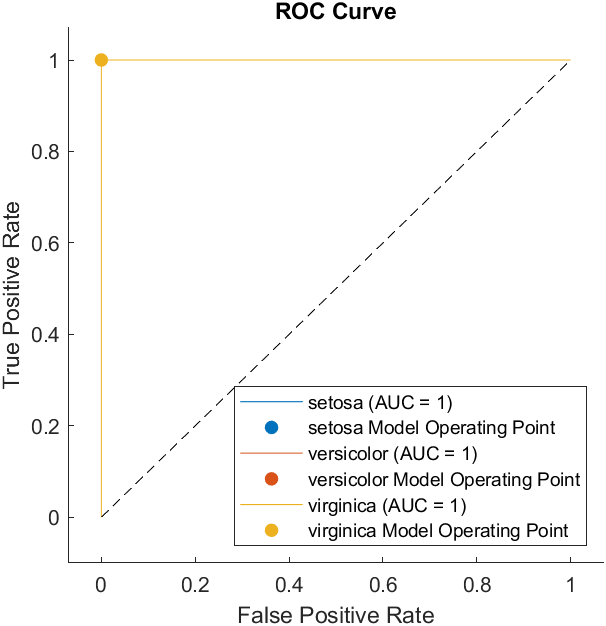
\includegraphics[width=0.8\linewidth]{figures/roc.png}
  \caption{ROC}
  \label{fig:boat1}
\end{figure}

\subsubsection{Validation and Testing Accuracy}

The effectiveness of our model is also confirmed by its high validation and testing accuracies. The model achieved a validation accuracy of 96.43\%, indicating its ability to correctly classify a high percentage of the validation dataset. More impressively, the model attained a testing accuracy of 100\%, suggesting that it performed exceptionally well on the unseen testing data.

\subsubsection{Visualization of Decision Boundaries}


\begin{figure}
  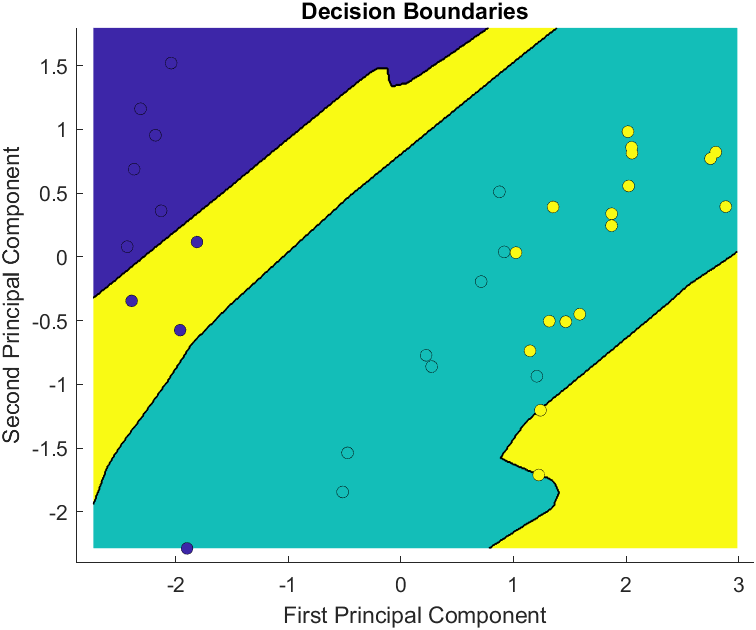
\includegraphics[width=\linewidth]{figures/DB.png}
  \caption{Decision Boundary}
  \label{fig:boat1}
\end{figure}

We visualized the decision boundaries of our model using Principal Component Analysis (PCA). This method allows us to project our multi-dimensional dataset into a 2D plane while preserving as much of the dataset's variation as possible. In our visualization, we colored the points corresponding to the Iris Virginica, Iris Versicolor, and Iris Setosa species in blue, teal, and yellow, respectively.

The resulting visualization showed that the decision boundary separating Iris Virginica from the other two species is well defined, suggesting that our model can easily differentiate Iris Virginica from the other two species. On the other hand, the decision boundary between Iris Versicolor and Iris Setosa appears to be more entangled, indicating some overlap in the characteristics of these two species. Despite this entanglement, our model still managed to achieve high accuracy, demonstrating its ability to learn complex patterns and make accurate classifications.



\subsubsection{Confusion Matrix}

Finally, we used a confusion matrix to provide a more detailed analysis of the model's performance. A confusion matrix is a table layout that visualizes the performance of an algorithm. Each row of the matrix represents the instances in an actual class, while each column represents the instances in a predicted class.

The confusion matrix for our model indicated only minor errors, suggesting that the model performed almost perfectly. This further confirms the model's robustness and ability to generalize well to unseen data. Overall, our model has demonstrated excellent performance in classifying the Iris species, underlining the effectiveness of our chosen architecture and training strategies.


\begin{figure}
  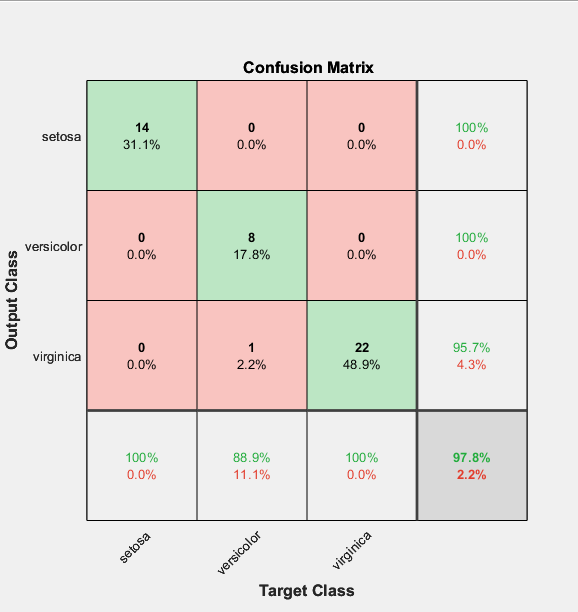
\includegraphics[width=0.7\linewidth]{figures/Cm.png}
  \caption{Confusion Matrix}
  \label{fig:boat1}
\end{figure}


\subsection{Conclusion}

In this study, we applied an Artificial Neural Network (ANN) to the Iris dataset classification problem, demonstrating the efficacy of such models in handling non-linearly separable data. The model achieved impressive accuracy on both validation and testing sets, further underscored by the perfect Area Under the Curve (AUC) of the Receiver Operating Characteristic (ROC) curve. Even with challenges such as the entanglement between Iris Versicolor and Iris Setosa, the model showcased a strong ability to classify instances correctly, evidenced by minor errors in the confusion matrix. This highlights the robustness of our model and its capacity to generalize well to unseen data.

For future work, it would be beneficial to experiment with varying network architectures, activation functions, and regularization techniques to further optimize the model Despite the inherent challenges of non-linear problems, our results demonstrate that with design, preprocessing, and optimization strategies, ANNs can deliver highly accurate and robust results.


\section{Part II: Genetic Algorithms for Global Optimization Problem}

\subsection{Function Selection and Analysis}

For the genetic algorithm section of our study, we've selected the Shubert function. This function, often used in optimization challenges, is characterized
by its complexity, featuring multiple local minima and maxima. This makes it an ideal choice for examining the robustness of genetic algorithms.

The Shubert function tests the algorithm's ability to navigate a landscape filled with local minima to find the global minimum. As the genetic algorithm
uses mechanisms inspired by natural evolution, it's well-suited for exploring a vast solution space.

Following this introduction, we'll provide details on the genetic algorithm's implementation, our chosen parameters, and the results of applying it to the
Shubert function, demonstrating its effectiveness in managing complex optimization problems.

\subsection{Genetic Algorithm Design}

\subsubsection{Representation of Initial Population}

\subsubsection{Fitness Function}

\subsubsection{Selection Method}

\subsubsection{Reproductive Operators}

\subsubsection{Stopping Criteria}

\subsubsection{Parameters and Constraints}
\subsection{GA Analysis of the Run}

\subsubsection{Selection Strategy}

\subsubsection{Comparison of Strategies}
\subsection{Results and Discussion}

\subsubsection{Premature Convergence}

\subsubsection{Maintaining Selection Pressure}

\subsubsection{Balancing Exploration and Exploitation}

\section{Conclusion}

\section*{References}


\bibliography{bib/IEEEabrv, bib/mybib}
\bibliographystyle{inc/IEEEtranS}


\end{document}